\chapter{Framework results}


\section{First test-run}
The first test-run were performed with 6 randomized constraints input to LegUp. This Each of the constraints could take the values 1 and 0, giving a total of $2^6=64$ combinations of constraints. The randomized constraints and the pattern of how the values are set is shown in \cref{tab:randomconstraint}.

\begin{table}
\tiny
    \begin{center}
    \begin{tabular}{l|cccccc}
     & & & \textbf{MB} & \textbf{ENABLE} & \textbf{DUAL} & \\
          &
          \textbf{SDC NO} & 
          \textbf{PIPELINE} & 
          \textbf{MINIMIZE} & 
          \textbf{PATTERN} & 
          \textbf{PORT} &
          \textbf{CASE} \\
        \textbf{Constraint}
           & \textbf{CHAINING}
           & \textbf{ALL}
           & \textbf{HW}
           & \textbf{SHARING}
           & \textbf{BINDING}
           & \textbf{FSM}
    \\ \midrule
    & 0 & 0 & 0 & 0 & 0 & 1 \\
    & 0 & 0 & 0 & 0 & 1 & 0 \\
    & 0 & 0 & 0 & 0 & 1 & 1 \\
    \textbf{Value} & \vdots & \vdots & \vdots & \vdots & \vdots & \vdots \\
    & &  &  &  &  &  \\
    & 1 & 1 & 1 & 1 & 1 & 0 \\
    & 1 & 1 & 1 & 1 & 1 & 1
    \\ \bottomrule
    \end{tabular}
    \caption{\label{tab:randomconstraint}Constraints and values for first run}
    \end{center}
\end{table}

The generated Verilog for many of the constraint files synthesize into the exact same area consumption and. This indicates that some of the constraints does not affect the generated Verilog in any way. The results are shown in \cref{tab:hlsrun1dataresults}. As there are only 8 different results, only $log_2(8) = 3$ constraint parameters affect the design, the other will be don't-care constraints. By converting the design number to binary, the first row of the result table is shown in \cref{tab:dectobinconstraints}, a pattern can be seen and that the parameters \textit{PIPELINE\_ALL}, \textit{ENABLE\_PATTERN\_SHARING} and \textit{DUAL\_PORT\_BINDING} are don't care for the this design.



\newcommand{\specialcell}[2][c]{%
  \begin{tabular}[#1]{@{}c@{}}#2\end{tabular}}
\begin{table}[hbtp]
    \centering
    \begin{tabular}{cccc}
    \textbf{Design \#} & \textbf{Area} & \specialcell{\textbf{Dynamic power}\\\textbf{[mW]}} & \specialcell{\textbf{Leakage power}\\\textbf{[nW]}} \\
    \toprule
    Verilog & 11660.582267 & 2.9522 & 13.2559 \\
    9,11,13,15,25,27,29,31 & 542636.067533 & 1.1933 & 445.5482  \\
    8,10,12,14,24,26,28,30 & 543715.713936 & 1.1909 & 442.7919 \\
    41,43,45,47,57,59,61,63 & 570759.857112 & 1.3097 & 474.8710 \\
    1,3,5,7,17,19,21,23 & 571069.521032 & 1.2792 & 467.3262 \\
    0,2,4,6,16,18,20,22 & 574368.902419 & 1.2745 & 467.3031 \\
    40,42,44,46,56,58,60,62 & 574468.505099 & 1.3100 & 475.3570 \\
    33,35,37,39,49,51,53,55 & 598731.305489 & 1.3951 & 498.4164 \\
    32,34,36,38,48,50,52,54 & 599552.442242 & 1.3949 & 500.0916 \\
    \bottomrule
    \end{tabular}
    \caption{Results from first framework run}
    \label{tab:llvmirparservectors}
\end{table}

\begin{table}[hbtp]
    \centering
    \begin{tabular}{cccc}
    \textbf{Decimal} & \textbf{Binary}\\
    \toprule
    9 & 001001 \\
    11 & 001011 \\
    13 & 001101 \\
    15 & 001111 \\
    25 & 011001 \\
    27 & 011011 \\
    29 & 011101 \\
    31 & 011111 \\
    \bottomrule
    \end{tabular}
    \caption{Decimal to binary conversion shows the pattern in the constraints}
    \label{tab:dectobinconstraints}
\end{table}


The results are visualized in \cref{fig:resultgraphhlsrun1}, together with the result of the same design written in Verilog directly. The data is sorted by area, showing the largest 

The best result with regards to area is the ones with the parameters \textit{SDC\_NO\_CHAINING} set to 0, \textit{MB\_MINIMIZE\_HW} set to 1 and \textit{CASE\_FSM} set to 1. The best result with regards to total power consumption is the same as for area, just with \textit{CASE\_FSM} set to 0.

\subsection{Criticism of the results}
It seems strange that the area consumption of the design written in Verilog is just 2.15\% of the best result from LegUp, while the power consumption of the design written in Verilog is 247.81\% of the best result from LegUp. Typically a larger design will consume more power, as each of the components has leakage and static operation consumption. Notice that this results were obtained using a static power estimation tool, the amount of switching in gates and registers has not been taken into account. However, this unexpected result has to be investigated further. The following steps must be taken to ensure that the results are correct:

\begin{itemize}
    \item Check generated reports for misinterpreted data
    \item Look at schematic view of synthesized design to 
    \item Run HLS and synthesis once more to see if results 
    \item Run toolflow using switching data to estimate power consumption
\end{itemize}


\begin{figure}[hbpt]
\centering
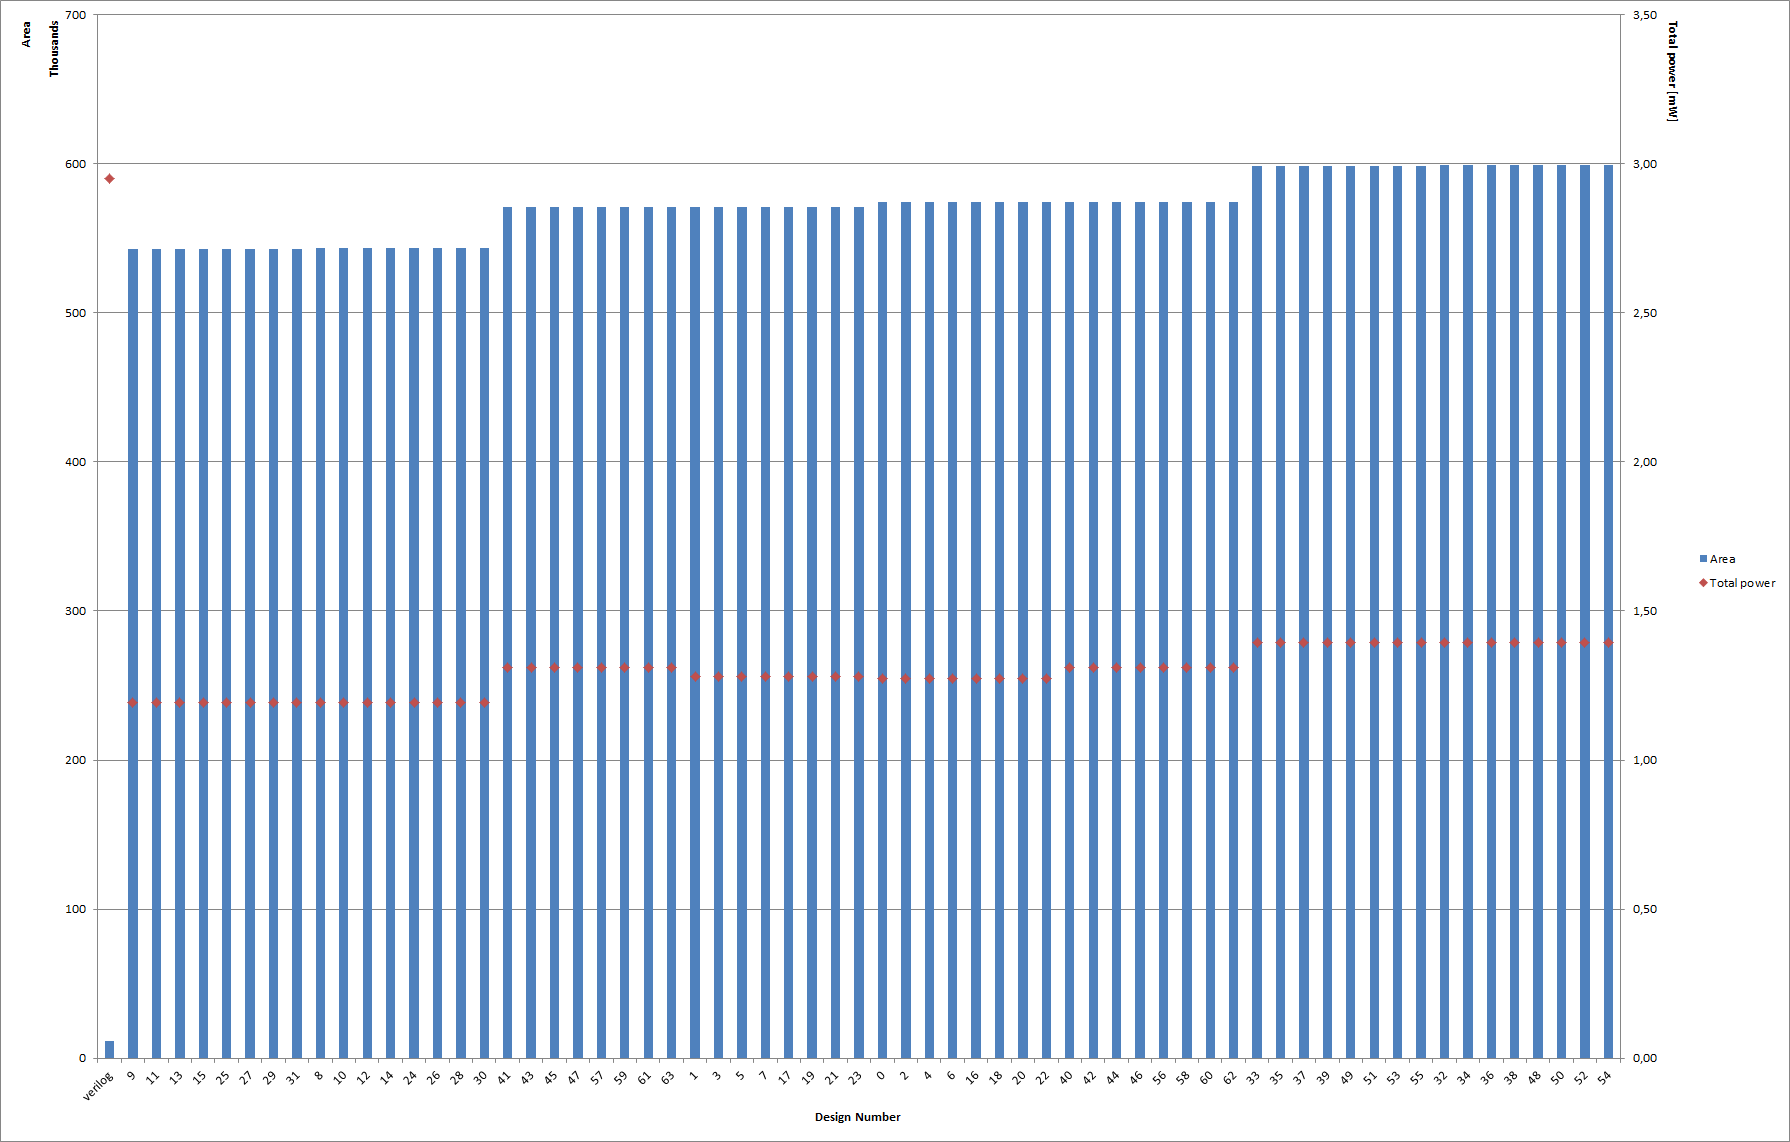
\includegraphics[width=\textwidth]{../figs/resultGraph.png}
\caption{\label{fig:resultgraphhlsrun1}Graph of results from first HLS run}
\end{figure}

\section{Path and hold violations}
Some of the designs reports violating path length and hold times in synthesis. For a real circuit this would be a problem. To get rid of these violations, the target clock speed during synthesis could be decreased to something below the maximum frequency of the design. However, the clock speed is most of the time the only thing you cannot change in your design, and design compiler will try to create the circuit that meets timing. If timing is not met, the circuit description should be changed. This means that from our methodology, we will generate many circuits and only the ones that meet timing will be presented as an accepted solution. Ideally, the framework would implement a feedback loop, but for the sake of this proof-of-concept, a long list of solutions are produced and only the best ones are selected.
